\documentclass[aspectratio=169]{beamer}


%%%%%%%%%%%%%%%%%%%%%%%%%%%%%%%%%%%%%%%%%%%%%%%%%%%%%
%%%%%%%%%%%%%%%%%%%%%%%%%%%%%%%%%%%%%%%%%%%%%%%%%%%%%
%%%%%%%%%%%%%%%%------ Package ------%%%%%%%%%%%%%%%%
%%%%%%%%%%%%%%%%%%%%%%%%%%%%%%%%%%%%%%%%%%%%%%%%%%%%%
%%%%%%%%%%%%%%%%%%%%%%%%%%%%%%%%%%%%%%%%%%%%%%%%%%%%%

\usepackage{amsmath,amssymb,amsfonts,amsthm}
\usepackage{cancel}
\usepackage{hyperref}
\usepackage{verbatim}
\usepackage{tabularx}
\usepackage{tikz}
\usepackage{dsfont}
\usepackage{mathtools}
\usepackage{bm}
\usepackage{epsfig}
%\usepackage[usenames,dvipsnames]{color}
\usepackage{graphicx}
\usepackage{url}
\usepackage{float}
\usepackage{epstopdf}
\usepackage{natbib}
\usepackage{bibentry}
\usepackage[titletoc]{appendix}
\usepackage{graphicx}
\usepackage{booktabs}
\usepackage{multirow, array}
\usepackage{ulem}
\usepackage{subfigure}
\usepackage{rotating}
\usepackage{blindtext}
\usepackage{todonotes}
\usepackage{tikz}

\setcounter{MaxMatrixCols}{10}


%%%%%%%%%%%%%%%%%%%%%%%%%%%%%%%%%%%%%%%%%%%%%%%%%%%%%
%%%%%%%%%%%%%%%%%%%%%%%%%%%%%%%%%%%%%%%%%%%%%%%%%%%%%
%%%%%%%%%%%%%%%%------- Theme -------%%%%%%%%%%%%%%%%
%%%%%%%%%%%%%%%%%%%%%%%%%%%%%%%%%%%%%%%%%%%%%%%%%%%%%
%%%%%%%%%%%%%%%%%%%%%%%%%%%%%%%%%%%%%%%%%%%%%%%%%%%%%

\mode<presentation>
{
    \usecolortheme{seagull}
    \usefonttheme{structuresmallcapsserif}
    \usefonttheme{serif}
    %\usefonttheme{professionalfonts}
    \usetheme{Pittsburgh}
    \setbeamercovered{dynamic}
    \setbeamertemplate{navigation symbols}{}
    \setbeamercolor{itemize item}{fg=gray} 
    \setbeamertemplate{itemize item}[ball]
    \setbeamercolor{itemize subitem}{fg=red!85!white}
    \setbeamertemplate{itemize subitem}[triangle]
    \setbeamertemplate{footline}[frame number]
}


%%%%%%%%%%%%%%%%%%%%%%%%%%%%%%%%%%%%%%%%%%%%%%%%%%%%%
%%%%%%%%%%%%%%%%%%%%%%%%%%%%%%%%%%%%%%%%%%%%%%%%%%%%%
%%%%%%%%%%%%%%%------- Theorem -------%%%%%%%%%%%%%%%
%%%%%%%%%%%%%%%%%%%%%%%%%%%%%%%%%%%%%%%%%%%%%%%%%%%%%
%%%%%%%%%%%%%%%%%%%%%%%%%%%%%%%%%%%%%%%%%%%%%%%%%%%%%

\theoremstyle{definition}
\newtheorem{defn}{\protect\definitionname}
\theoremstyle{plain}
\newtheorem{conjecture}{\protect\conjecturename}
\theoremstyle{plain}
\newtheorem{claim}{Claim}
\theoremstyle{definition}
%% \newtheorem{ax}{\protect\axiomname}
\theoremstyle{plain}
\newtheorem{thm}{\protect\theoremname}
\theoremstyle{plain}
\theoremstyle{plain}
\newtheorem{cor}{\protect\corollaryname}
\theoremstyle{plain}
\newtheorem{proposition}{\protect\propositionname}
\theoremstyle{remark}
\newtheorem{rem}{Remark}
\theoremstyle{definition}
\newtheorem{observation}{Observation}
  
\providecommand{\axiomname}{Axiom}
\providecommand{\conjecturename}{Conjecture}
\providecommand{\definitionname}{Definition}
\providecommand{\corollaryname}{Corollary}
\providecommand{\theoremname}{Theorem}
\providecommand{\propositionname}{Proposition}

\title{Tailored Stories}
\author{Author: Chiara Aina \\ \vspace{0.8cm} \\ Presenter: Sayantan Roy, Zhongheng Qiao, Omaretsoguwa Atsagbede}
\date{\today}

\begin{document}

\begin{frame}
  \maketitle
\end{frame}

\section{Motivation}

\begin{frame}{Narratives Matter}
Different narratives lead to different conclusions
  \begin{itemize}
    \item Voters may disagree on the outcome of an election \\ 
     \textcolor{gray}{\small "The election system is fair" vs. "Elections are rigged"}
    \item Consumers often differ in evaluating a company \\
     \textcolor{gray}{\small "This company has great CSR" vs. "The company is just greenwashing"}
    \item Investors make different predictions based on past financial data \\
      \textcolor{gray}{\small "What goes down comes up" vs. "Early success predicts long-run success"}
  \end{itemize}
\end{frame}

\begin{frame}{This Paper}
To which extent is possible to manipulate beliefs with narratives (models)?
  \begin{enumerate}
    \item Without controlling the information to be observed
    \item Without knowing the information to be interpreted 
  \end{enumerate}
  
  \begin{itemize}
    \item Main result characterizes the extent of belief manipulability
    \item The agent might hold inconsistent beliefs across contingencies
    \item Extent to which the agent is vulnerable to persuasion depends on initial beliefs
    \item Belief polarization is inevitable with conflicting narratives
  \end{itemize}
\end{frame}


\begin{frame}{Set-Up}
  \begin{center}
    \includegraphics[width=.8\textwidth]{fig_intro/fig1.jpg}
  \end{center}
\end{frame}

\begin{frame}{Timeline}
  \begin{center}
    \includegraphics[width=.8\textwidth]{fig_intro/fig2.jpg}
  \end{center}
\end{frame}

\begin{frame}{Timeline}
  \begin{center}
    \includegraphics[width=.8\textwidth]{fig_intro/fig3.jpg}
  \end{center}

\end{frame}
\begin{frame}{Timeline}

  \begin{center}
    \includegraphics[width=.8\textwidth]{fig_intro/fig4.jpg}
  \end{center}
 \end{frame}



%%%%%%%%%%%%%%%%%%%%%%%%%%%%%%%%%%%%%%%%%%%%%%%%%%%%%
%%%%%%%%%%%%%%%%%%%%%%%%%%%%%%%%%%%%%%%%%%%%%%%%%%%%%
%%%%%%%%%%%%------- Part 2 Slides -------%%%%%%%%%%%%
%%%%%%%%%%%%%%%%%%%%%%%%%%%%%%%%%%%%%%%%%%%%%%%%%%%%%
%%%%%%%%%%%%%%%%%%%%%%%%%%%%%%%%%%%%%%%%%%%%%%%%%%%%%
\section{Main Results}

\begin{frame}[label=EN1]{Environment}
    \begin{itemize}
        \item Two agents: Sender (S) and Receiver (R)
        \smallskip
        \begin{itemize}
            \item State space \( \omega \in \Omega \); signal space \( s \in S \); receiver's action space \( a \in A\)
            \item  common prior \(\mu_0 \in int(\Delta(\Omega))\); utility function \( U^{S/R} (a, \omega) \)
        \end{itemize}
        \bigskip
        \item Model \( m \in \mathcal{M} \): \( \Omega \rightarrow \Delta(S) \)
        \smallskip
        \begin{itemize}
            \item A model \( m \) maps a distribution of signals to each state (\textit{interpretation} of signals): \[ \sum_{s \in S} \pi^m(s|\omega) = 1, \ \forall \omega \in \Omega \]
            \item A model \( m \) needs to interpret all possible signals: \[ \forall s \in S, \ \exists \ \omega \ s.t. \ \pi^m(s|\omega) > 0 \]
            \item A model \( m \) induces posterior belief \( \mu^m_s \) via Bayes rule: 
            \[\mu^m_s(\omega\mid s) = \frac{\mu_0(\omega) \pi^m(s|\omega)}{Pr^m(s)}\]
        \end{itemize}
    \end{itemize}
\end{frame}

\begin{frame}[label=PB1]{Vectors of Posterior Beliefs}

Let \( \bm{\mu} = (\mu_s)_{s \in S} \in [\Delta(\Omega)]^S \) represent a vector of posterior beliefs: an array of posterior distributions conditional on each signal

\begin{columns}[c] 	
	\column{.47\textwidth} % Left column and width
	\begin{center} 
		\def\myscale{1}
		\scalebox{\myscale}[\myscale]{
			\begin{tikzpicture}[xscale=4.8,yscale=4.8]
				\draw [opacity=.75] (-.01,-.01) -- (1.01,-0.01) -- (1.01, 1.01) -- (-.01, 1.01) -- (-.01, -.01);
				
				\foreach \x in {0.2, 0.4, 0.6, 0.8}
				{
					\draw [opacity=.75] (\x,-.01) -- (\x, 0);
					\draw [opacity=.75] (\x,1.01) -- (\x,1);
				}

                \foreach \x in {0, 0.2, 0.4, 0.6, 0.8, 1}
                {
                    \node at (\x, -.07) {\scriptsize\x};
                }
				
				\foreach \y in {0, 0.2, 0.4, 0.6, 0.8}
				{
					\draw [opacity=.75] (-.01,\y) -- (0,\y);
					\draw [opacity=.75] (1.01,\y) -- (1,\y);
				}

                \foreach \y in {0, 0.2, 0.4, 0.6, 0.8, 1}
                {
                    \node at ( -.09, \y) {\scriptsize\y};
                }
				
				\node at (0.51,-0.15) { \footnotesize \( \Pr (B|W) \) };
				\node [rotate=90] at (-0.2, 0.51) { \footnotesize \( \Pr (B|\lnot{W}) \) };

                %%% Above is default figure %%%

                \only<2->{
                \draw [dashed, opacity=.5] (-.01, .7) -- (1.01, .7);
                \draw [dashed, opacity=.5] (.7, -.01) -- (.7, 1.01);
                \draw [fill=orange] (.7, .7) circle (.015);
                }

                \only<3->{
                \draw [dashed, opacity=.5] (-.01, 0) -- (1.01, 0);
                \draw [dashed, opacity=.5] (1, -.01) -- (1, 1.01);
                \draw [fill=red] (1, 0) circle (.015);
				}
		  \end{tikzpicture}}
	\end{center} 
		
	\column{.47\textwidth} % Right column and width
	\begin{itemize}
            \item Axis: posterior of \( B \) conditional on each signal
            \item Every model induces a vector of posteriors
            \item<2-> Orange point: prior on B = 0.7
            \item<3-> Red point: vectors of posteriors by fair model
    \end{itemize}
\end{columns}
\end{frame}

\begin{frame}[label=PB2]{Vectors of Posterior Beliefs}

\begin{definition}[Bayes-consistency]
    A vector of posterior beliefs \( \bm{\mu} \) is \textit{Bayes-consistent} if the prior is a strict convex combination of the posteriors across signals: \( \exists \  \varphi \in \int(\Delta(S)) \ s.t. \ \mu_0 = \sum_{s \in S} \varphi_s \mu_s \)
\end{definition}

\begin{columns}[c] 	
	\column{.47\textwidth} % Left column and width
	\begin{center} 
		\def\myscale{1}
		\scalebox{\myscale}[\myscale]{
			\begin{tikzpicture}[xscale=4,yscale=4]
				\draw [opacity=.75] (-.01,-.01) -- (1.01,-0.01) -- (1.01, 1.01) -- (-.01, 1.01) -- (-.01, -.01);
				
				\foreach \x in {0.2, 0.4, 0.6, 0.8}
				{
					\draw [opacity=.75] (\x,-.01) -- (\x, 0);
					\draw [opacity=.75] (\x,1.01) -- (\x,1);
				}

                \foreach \x in {0, 0.2, 0.4, 0.6, 0.8, 1}
                {
                    \node at (\x, -.07) {\scriptsize\x};
                }
				
				\foreach \y in {0, 0.2, 0.4, 0.6, 0.8}
				{
					\draw [opacity=.75] (-.01,\y) -- (0,\y);
					\draw [opacity=.75] (1.01,\y) -- (1,\y);
				}

                \foreach \y in {0, 0.2, 0.4, 0.6, 0.8, 1}
                {
                    \node at ( -.09, \y) {\scriptsize\y};
                }
				
				\node at (0.51,-0.15) { \footnotesize \( \Pr (B|W) \) };
				\node [rotate=90] at (-0.2, 0.51) { \footnotesize \( \Pr (B|\lnot{W}) \) };

                \draw [fill=orange] (.7, .7) circle (.015);

                \only<1>{
                \draw [dashed, opacity=.5] (-.01, .7) -- (1.01, .7);
                \draw [dashed, opacity=.5] (.7, -.01) -- (.7, 1.01);
                }
				
				\only<2->{
                \draw [draw=none,fill=violet,opacity=.25] (-.01, .7) -- (.7, .7) -- (.7, 1.01) -- (-.01, 1.01);
                \draw [draw=none,fill=violet,opacity=.25] (.7, .7) -- (.7, -.01) -- (1.01, -.01) -- (1.01, .7);
                }
		\end{tikzpicture}}
	\end{center} 
		
	\column{.47\textwidth} % Right column and width
	\begin{itemize}
            \item<2-> Equivalent representation between models and Bayes-consistent vectors of posteriors:
            \smallskip
            \begin{itemize}
                \item Each Bayes-consistent vector of posteriors \( \bm{\mu} \in \mathcal{B} \) could be induced by a model
                \item Each model \( m \) induces a Bayes-consistent vector of posteriors
            \end{itemize}
        \end{itemize}
\end{columns}

\end{frame}

\begin{frame}[label=PB3]{Feasible Posterior Beliefs: One Model}

\begin{proposition}[One Model]
    If \( |M| = 1 \), the set of feasible vectors of posteriors equals \( \mathcal{B} \), the set of all Bayes-consistent vectors of posteriors.
\end{proposition}

\begin{columns}[c] 	
	\column{.47\textwidth} % Left column and width
	\begin{center} 
		\def\myscale{1}
		\scalebox{\myscale}[\myscale]{
			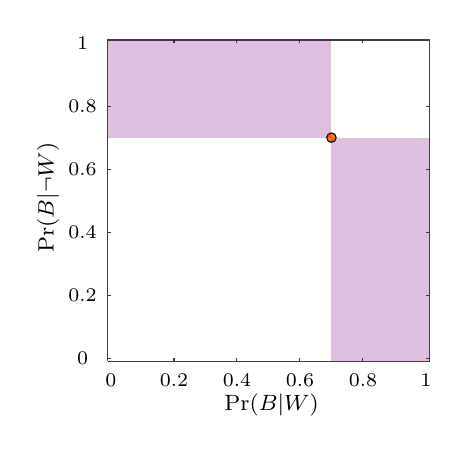
\begin{tikzpicture}[xscale=4,yscale=4]
				\draw [opacity=.75] (-.01,-.01) -- (1.01,-0.01) -- (1.01, 1.01) -- (-.01, 1.01) -- (-.01, -.01);
				
				\foreach \x in {0.2, 0.4, 0.6, 0.8}
				{
					\draw [opacity=.75] (\x,-.01) -- (\x, 0);
					\draw [opacity=.75] (\x,1.01) -- (\x,1);
				}

                \foreach \x in {0, 0.2, 0.4, 0.6, 0.8, 1}
                {
                    \node at (\x, -.07) {\scriptsize\x};
                }
				
				\foreach \y in {0, 0.2, 0.4, 0.6, 0.8}
				{
					\draw [opacity=.75] (-.01,\y) -- (0,\y);
					\draw [opacity=.75] (1.01,\y) -- (1,\y);
				}

                \foreach \y in {0, 0.2, 0.4, 0.6, 0.8, 1}
                {
                    \node at ( -.09, \y) {\scriptsize\y};
                }
				
				\node at (0.51,-0.15) { \footnotesize \( \Pr (B|W) \) };
				\node [rotate=90] at (-0.2, 0.51) { \footnotesize \( \Pr (B|\lnot{W}) \) };

                \draw [fill=orange] (.7, .7) circle (.015);
                \draw [draw=none,fill=violet,opacity=.25] (-.01, .7) -- (.7, .7) -- (.7, 1.01) -- (-.01, 1.01);
                \draw [draw=none,fill=violet,opacity=.25] (.7, .7) -- (.7, -.01) -- (1.01, -.01) -- (1.01, .7);
		\end{tikzpicture}}
	\end{center} 
		
	\column{.47\textwidth} % Right column and width
	\begin{itemize}
            \item Only Bayes-consistent vectors of posterior beliefs are feasible when a single model is proposed
        \end{itemize}
\end{columns}
\end{frame}

\begin{frame}[label=EN2]{Model Adoption}
    \begin{itemize}
        \item Fit of a model \( m \) conditional on the signal \( s \): \[ \textstyle{\Pr^m(s)} = \sum\limits_{\omega \in \Omega} \mu_0(\omega) \pi^m(s|\omega)\]
        \smallskip
        \item After the sender sends a set of model \( M \subseteq \mathcal{M} \):
        \smallskip
        \begin{itemize}
            \item The receiver adopts \(m^* \in M \) that best fits signal \( s \): \[ m^* \in \arg\max_{m \in M} \textstyle{\Pr^m(s)}\]
            \item The receiver updates her prior via Bayes rule and chooses the action that maximizes her expected utility calculated using model \( m^* \)
        \end{itemize}
    \end{itemize}
\end{frame}

\begin{frame}{Model Adoption: Many Models}
When the sender sends a set of models \( M \in \mathcal{M} \), the receiver adopts the model with the highest fit given the signal

\begin{columns}[c] 	
	\column{.47\textwidth} % Left column and width
	\begin{center} 
		\def\myscale{1}
		\scalebox{\myscale}[\myscale]{
			\begin{tikzpicture}[xscale=4.8,yscale=4.8]
				\draw [opacity=.75] (-.01,-.01) -- (1.01,-0.01) -- (1.01, 1.01) -- (-.01, 1.01) -- (-.01, -.01);
				
				\foreach \x in {0.2, 0.4, 0.6, 0.8}
				{
					\draw [opacity=.75] (\x,-.01) -- (\x, 0);
					\draw [opacity=.75] (\x,1.01) -- (\x,1);
				}

                \foreach \x in {0, 0.2, 0.4, 0.6, 0.8, 1}
                {
                    \node at (\x, -.07) {\scriptsize\x};
                }
				
				\foreach \y in {0, 0.2, 0.4, 0.6, 0.8}
				{
					\draw [opacity=.75] (-.01,\y) -- (0,\y);
					\draw [opacity=.75] (1.01,\y) -- (1,\y);
				}

                \foreach \y in {0, 0.2, 0.4, 0.6, 0.8, 1}
                {
                    \node at ( -.09, \y) {\scriptsize\y};
                }
				
				\node at (0.51,-0.15) { \footnotesize \( \Pr (B|W) \) };
				\node [rotate=90] at (-0.2, 0.51) { \footnotesize \( \Pr (B|\lnot{W}) \) };

                \draw [fill=orange] (.7, .7) circle (.015);
                \draw [fill=red] (1, 0) circle (.015);
                \draw [fill=blue] (.04, .82) circle (.015);
                \draw [draw=none,fill=violet,opacity=.25] (-.01, .7) -- (.7, .7) -- (.7, 1.01) -- (-.01, 1.01);
                \draw [draw=none,fill=violet,opacity=.25] (.7, .7) -- (.7, -.01) -- (1.01, -.01) -- (1.01, .7);

                \only<2->{
                \draw [color=red, thick] (.569, 1.01) -- (1,0);
                \draw [color=blue, thick] (0, 0.827) -- (1.01, .6449);
                }
				
				\only<3->{
                \draw [dashed, opacity=0.75] (0, 0.82) -- (1, 0.82);
                \draw [dashed, opacity=0.75] (1, 0) -- (1, 1);
                \draw [fill=black] (1, 0.82) circle (.015);
                }
		\end{tikzpicture}}
	\end{center} 
		
	\column{.47\textwidth} % Right column and width
	\begin{itemize}
            \item<2-> Isofit line: all the points whose models have the same fit:
            \begin{itemize}
                \item The steeper, the higher fit given signal \( W \)
                \item The flatter, the higher fit given signal \( \lnot W \)
            \end{itemize}
            \smallskip
            \item<3-> Given signal \( W \), the \textcolor{red}{fair model} is adopted
            \item<3-> Given signal \( \lnot{W} \), the \textcolor{blue}{conspiracy model} is adopted
        \end{itemize}
\end{columns}
\end{frame}

\begin{frame}[label=PB4]{Feasible Posterior Beliefs: Many Models}

\begin{itemize}
    \item Vector of posterior beliefs: \( \bm{\mu} = (\mu_s)_{s \in S} \in [\Delta(\Omega)]^S \)
    \smallskip
    \item Maximal movement for \( \mu_s \): \( \bar{\delta}(\mu_s) = \max\limits_{\omega \in \Omega} \frac{\mu_s(\omega)}{\mu_0(\omega)} \)
    \begin{itemize}
        \item Measures of how much the target posterior is far from the prior
    \end{itemize}
    \smallskip
    \item \( H \) represents the harmonic mean of a vector
    \begin{itemize}
        \item Let \( x = (x_1,...,x_N) \), \( H(x) = (\sum_{i=1}^N x_i^{-1}/N )^{-1} \)
    \end{itemize}
    \medskip
\end{itemize}

\begin{theorem}[Many Model]
    The set of feasible vectors of posteriors is \( \mathcal{F} = \Big\{ \bm{\mu} \in [\Delta(\Omega)]^S: H(\bar{\delta}(\mu_s)) \leq |S| \Big\} \)
\end{theorem}

\begin{itemize}
    \item The intuition is: on average, the feasible vector of posteriors should not be too far away from the prior
\end{itemize}

\end{frame}

\begin{frame}[label=PB5]{Feasible Posterior Beliefs: Many Models}

Full characterization of the set of feasible vectors of posteriors: on average, the posteriors across signals should not be too far away from the prior

\begin{columns}[c] 	
	\column{.47\textwidth} % Left column and width
	\begin{figure}
		\includegraphics[height=0.8\textwidth]{Figs/Fig_05.PNG}
	\end{figure}
		
	\column{.47\textwidth} % Right column and width
	\begin{itemize}
            \item Bayes-inconsistent vectors of posteriors could be induced
            \item Not all vectors of posteriors are feasible
        \end{itemize}
\end{columns}

\end{frame}

%%%%%%%%%%%%%%%%%%%%%%%%%%%%%%%%%%%%%%%%%%%%%%%%%%%%%
%%%%%%%%%%%%%%%%%%%%%%%%%%%%%%%%%%%%%%%%%%%%%%%%%%%%%
%%%%%%%%%%%%------- Part 3 Slides -------%%%%%%%%%%%%
%%%%%%%%%%%%%%%%%%%%%%%%%%%%%%%%%%%%%%%%%%%%%%%%%%%%%
%%%%%%%%%%%%%%%%%%%%%%%%%%%%%%%%%%%%%%%%%%%%%%%%%%%%%
\section{Application}

\begin{frame}
  \vfill
  \centering
  \textbf{Details Supporting The Main Findings (Applications Of Findings)}
  \vfill
\end{frame}


\begin{frame}{Firehose Of Falsehood}
  \textbf{Firehose Of Falsehood:} \\
  \vspace{0.3cm} % Adjust space as needed
  \begin{itemize}
    \item A quick explanation of the strategy known as the \textbf{Firehose of Falsehood}, which involves \textbf{overwhelming people} with a \textbf{high volume of conflicting messages}, making it hard to know the difference between true and false information.
  \end{itemize}
  \vspace{0.3cm}
  \begin{itemize}
    \item An example is about how this approach can influence voters during an election, leading them to form \textbf{polarized beliefs} based on \textbf{different narratives}.
  \end{itemize}
  \vspace{0.3cm} % Adjust space as needed
  \textcolor{gray}{\small Figure 3 shows this with different probabilities that voters assign to the legitimacy of an election based on their priors.}
\end{frame}


\begin{frame}{Election Narratives and Voter Perception}
  \begin{figure}
      \centering
      \includegraphics[width=1\linewidth]{image.png}
      \label{fig:enter-label}
  \end{figure}
\end{frame}


\begin{frame}{}
  \begin{itemize}
    \item \textbf{Question:} How conflicting informational models affect people's beliefs about political events (like election legitimacy), specifically regarding the conditions under which beliefs become polarized.
  \end{itemize}
\end{frame}



\begin{frame}{Model Polarization}
  \begin{theorem}[Binary Case, Polarization]
  For each pair of conflicting models, there exists a threshold $p$ such that, for every signal $s$, it holds that [(i)]
\item $\mu_s(\omega_1) > \mu_0(\omega_1)$ if $\mu_0(\omega_1) < p$, and 
\item $\mu_s(\omega_1) < \mu_0(\omega_1)$ if $\mu_0(\omega_1) > p$.
\end{theorem}
    \item The intuition is the following: Any pair of conflicting models induces a vector of posteriors that is not Bayes-consistent, with both posteriors higher or lower than the prior.
    
\end{frame}

\begin{figure}
    \centering
    \includegraphics[width=0.6\linewidth]{AccuracyOfVoteCount.png}
    \caption{Figure 4: Accuracy of vote count (Persily and Stewart, 2021)
Notes: The y-axis shows the percentage answering “a great deal” or “quite a bit” in response to the question “How much confidence do you have that your vote in the 2020 presidential election [will be/was] counted accurately?” Source: Economist/YouGov poll, 2020.}
    \label{}
\end{figure}

\begin{frame}{Firehose of Falsehood}
  \begin{itemize}
    \item The fair model is adopted if
    \[
      \operatorname{Pr}^F(W) > \operatorname{Pr}^C(W)
    \]
    \item Calculate for which prior \( p \) this is the case:
    \begin{gathered}
      p \cdot 99\% + (1-p) \cdot 1\% \geq p \cdot 1\% + (1-p) \cdot 50\% \\
      p \geq 33\%
    \end{gathered}
  \end{itemize}
\end{frame}

\begin{frame}{Explanation}
  \begin{itemize}
    \item There's a certain threshold probability $p$. 
    \item If a person's initial belief about a situation (prior probability) is less than $p$, any new information will likely decrease their belief.
    \item If their initial belief is greater than $p$, new information will likely increase their belief. 
    \item This occurs when the information models (signals) are conflicting.
    \item When people are given conflicting information, the way they update their beliefs is not always rational (not Bayes-consistent), leading to beliefs that are either all higher or all lower than what they initially thought.
  \end{itemize}
  \vspace{0.5cm}
  This can be viewed more into context in \textbf{The Case of the 2020 US Presidential Election}.
\end{frame}

\begin{frame}{Firehose of Falsehood: 2020 US Presidential Elections}
  \begin{itemize}
    \item Predictions: when exposed to conflicting models...
    \begin{enumerate}
      \item Voters with different priors adopt different models once the outcome is observed
      \item Voters with similar priors adopt different models once observed different outcomes
    \end{enumerate}
    \item Assumption: voters expect their partisan candidate to win
    \begin{itemize}
      \item Republicans expect Trump to win
      \item Democrats expect Biden to win
    \end{itemize}
  \end{itemize}
\end{frame}



\begin{figure}
    \centering
    \includegraphics[width=0.8\linewidth]{PresentationImage.png}
    \label{fig:enter-label}
\end{figure}



%%%%%%%%%%%%%%%%%%%%%%%%%%%%%%%%%%%%%%%%%%%%%%%%%%%%%
%%%%%%%%%%%%%%%%%%%%%%%%%%%%%%%%%%%%%%%%%%%%%%%%%%%%%
%%%%%%%%%%%%------- Optional Page -------%%%%%%%%%%%%
%%%%%%%%%%%%%%%%%%%%%%%%%%%%%%%%%%%%%%%%%%%%%%%%%%%%%
%%%%%%%%%%%%%%%%%%%%%%%%%%%%%%%%%%%%%%%%%%%%%%%%%%%%%
\section{Appendix}

\begin{frame}{}
    \centering \Huge
    \emph{Thank You!}
\end{frame}

\begin{frame}[label=RP]{Receivers' Vulnerability to Persuasion}
\end{frame}

\begin{frame}[label=SP]{Senders' Problem}
\end{frame}

\begin{frame}[label=SP]{More Applications}
  \begin{itemize}
    \item \textbf{Financial Advice:} conflict of interest in finance between a financial advisor and an investor with private information (past experience)
      \begin{itemize}
        \item The advisor can manipulate the investor regardless of her private signal, always moving her beliefs in the advantageous direction
      \end{itemize}
    \item \textbf{Lobbying:} challenge a well-established way of looking at scientific evidence, so-called ``Merchants of Doubt'' (e.g., Michaels, 2008; Oreskes \& Conway, 2011)
      \begin{itemize}
        \item Given a shared default model (trust in science), it is still possible to insinuate doubt
      \end{itemize}
    \item \textbf{Self-Persuasion:} an agent can distort her own beliefs by manipulating the perceived informativeness of observable signals
      \begin{itemize}
        \item Leaving facts open to interpretation can be used to achieve self-serving beliefs
        \item Distorting confidence using models can motivate in committing to a costly action
      \end{itemize}
  \end{itemize}
\end{frame}

\end{document}
